% !TEX TS-program = xelatex
% !TEX encoding = UTF-8

% This is a simple template for a XeLaTeX document using the "article" class,
% with the fontspec package to easily select fonts.

\documentclass{ctexart} % 使用ctex 适配过的article 文档类

%\usepackage{fontspec} % Font selection for XeLaTeX; see fontspec.pdf for documentation
%\defaultfontfeatures{Mapping=tex-text} % to support TeX conventions like ``---''
%\usepackage{xunicode} % Unicode support for LaTeX character names (accents, European chars, etc)
%\usepackage{xltxtra} % Extra customizations for XeLaTeX
% other LaTeX packages.....
\usepackage{geometry} % See geometry.pdf to learn the layout options. There are lots.
\geometry{a4paper} % or letterpaper (US) or a5paper or....
%\usepackage[parfill]{parskip} % Activate to begin paragraphs with an empty line rather than an indent

\usepackage{graphicx} % support the \includegraphics command and options
\graphicspath {{fig/}} % 设置图片目录
\usepackage{cite}

%\usepackage{minted} %You must invoke LaTeX with the -shell-escape flag.

\title{交流架空线路的电磁环境}
\author{张庭梁  刘寒玉  李明轩}
\date{Today} % Activate to display a given date or no date (if empty),
         % otherwise the current date is printed 

\begin{document}
\maketitle
摘要:随电网规模的不断扩大和输电电压等级的不断提高,输电线路的电磁环境影响越来越受到关注。交流输电线路对环境的影响从电磁角度分析,主要有工频电、磁场,无线电干扰,电晕噪声等,城市建设规划和环保执法中对工频电磁场尤其关注。

高压输电在实现电力有效配置中发挥着重要作用,这是中国经济快速发展的前提之一。然而,传输线中的高压也会在它们周围产生电磁场,这可能会影响人们的健康和附近设备的功能。

本文主要介绍输电线路周围的电磁环境。首先,提到了与电场强度和磁场强度相关的几个因素。其次,根据这些因素,还介绍了一些减小电磁场影响的方法。此外,有几种情况可以证明这些方法的有效性。

关键词:电磁环境,高压输电,电场,磁场

%\tableofcontents % 这里是目录

\section{备受关注的输电线路电磁环境问题}

近年来,由输变电工程电磁环境引发的问题越来越突出,在全国各地不断有居民上访、阻挠施工、到供电部门静坐等情况出现。究其原因主要有以下几方面: 

\begin{enumerate}
\item 
缺乏强制性的国家标准。高压输变电工程电、磁场问题(特别是工频电磁场) 的国家标准的研究工作正在进行,目前针对高压线路电、磁场书面的、公开颁布的行业规范是《500 kV 超高压送变电工程电磁辐射环境影响评价技术规范》( HJ /T24 - 1998) 《110~500 kV 架空送电线路设计技术规范》(DL/ T 5092 - 1999) 中也有关于工频电场限值的规定;
\item 
电力建设规划与城市建设规划的不同步。电力建设从规划到建成需要较长一段时间,当1 个电力建设项目完成规划、设计、审批后,在建设过程中,由于城市建设规划的改变,一些原来建于城市周边的高压线等电力设施周围也开始进行开发,导致新的问题; 
\item
 由于人们对电磁场或电磁波的特性不了解,尤其对输变电工程产生的工频电、磁场的误解,把高压输电线与电磁“辐射”甚至与核辐射联系起来;
\item
生活小区的不规范建设。
\end{enumerate}

\section{输电线路周围的电磁环境的计算}

尽管电力需求和能源分配不均衡,为实现我国能源资源的优化配置,推进特高压电网建设势在必行,可以促进电能的可持续发展,减轻环境污染。然而,随着人们对健康和环境保护意识的不断提高,特高压输电的电磁污染引起了公众的关注和关注。对电磁环境的研究相对较少,不能满足人们对环境影响的深入研究需求。因此,本文重点研究高压输电线路周围的电磁环境。

本文提出了几种方法,包括电荷模拟方法,Biot-Savart定律分析方法等。为了保证本文的科学可读性和普及性,可以在最后一页的参考资料中找到一些详细的计算方法。有些人担心中国的高压输电电磁污染。本文将重点关注电磁环境的评估,提供高压传输的清晰轮廓,消除对高压传输的误解。

本节首先分析了高压输电线路上的电场,主要关注与电场强度有关的几个因素。由于空间的限制,本文仅关注两个因素 - 传输线的高度和布局。然后是磁场部分,还关注了与磁场强度相关的因素。

\subsection{ 超高压输电线路工频电场分析}

由于需要降低变换期间的功率损耗,变换线上的电压已达到一定的高水平。当电压高于1000kV时,通常称为超高压或UHV。当超高压输电线路工作时,导线上的电荷将在空间产生工频电场。有几个因素决定了电场强度,如传输线的高度,传输线的布局等。在传输线的构建过程中,优化电缆的布局可以极大地减少电场和磁场的影响,最大限度地减少传输线对附近人员和机器的影响。



\subsubsection{高度对工频电场的影响}

为了分析高度对电场产生的电场的影响,我们假设传输线无限长并且平行于地面,这可以被认为是良导体。在假设下,我们可以使用电荷模拟方法来计算传输线上的等效电荷。并且在我们得到每单位长度的等效有效电荷之后,可以根据叠加原理计算空间中任何点的电场强度。具体计算基于张可心的论文“超高压输电线路电磁环境研究(2009)\cite{张可心2009超高压传输线电磁环境特性研究}”。

在计算的基础上,我们可以判断传输线高度对地面电场强度的影响。图~\ref{1}清楚地显示了它。地面电场强度随着导体接地高度的增加而减小。这种关系可用于减少传输线对地的影响。图~\ref{1}显示了不同高度的最高电场强度。根据中国对居民区输电线路最大电场强度的要求,最高电场强度应不大于4kV / m,表明输电线路高度应大于14 m。然而,在施工过程中,我们应该考虑由于重力引起的输电线路下垂,这意味着我们应该将输电线路的高度提高得更高。
\begin{figure}[htbp]
\small
\centering
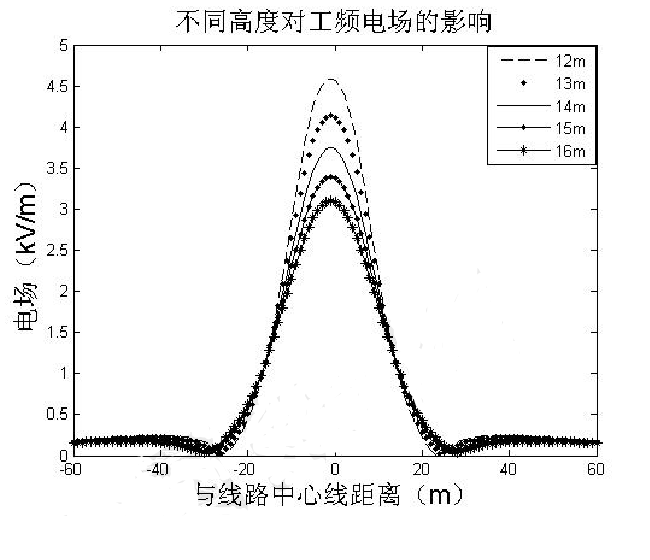
\includegraphics[width=8cm]{1.png}
\caption{高度对工频电场的影响} 
\label{1}
\end{figure}


表1:不同高度的最高电场强度

高度(m)12 13 14 15 16

电场强度(kV / m)4.589 4.136 3.725 3.383 3.091


\subsubsection{传输线布局对电场的影响}
在研究和实践的基础上,不同的输电线路布局会导致不同的电场。北京交通大学电气工程学院徐杨认为,当线路垂直放置时,场强分布将达到顶峰\cite{许杨2007高压输电线路工频电磁环境}。然而,水平布局导致高强度电场的最大覆盖区域。如果三相线以倒三角形排列,则电场的最大值和覆盖面积都将最大程度地减小。目前的输电塔形式证明了徐的理论。

根据不同的输电线路布局,有不同种类的输电塔,如杯型塔,紧凑型塔等,如图~\ref{1}。在杯型塔中,三相线以三角形排列,而在紧凑型塔中,它呈倒三角形。基于与徐一样的计算,陈博栋发现杯型塔周围的电场强度高于紧凑型塔的电场强度,这在他的论文“电磁环境的数值模拟研究\cite{陈博栋2015特高压输电线路电磁环境数值模拟研究} ”中有所体现。

\begin{figure}[htbp]
\small
\centering
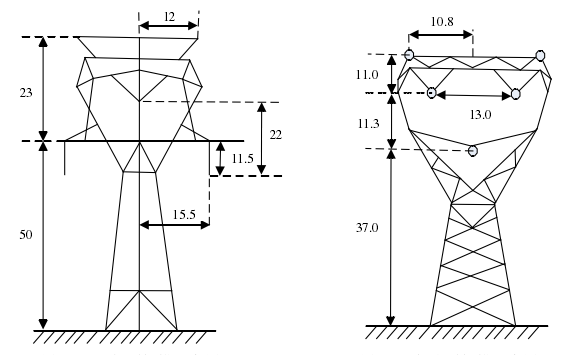
\includegraphics[width=8cm]{2.png}
\caption{杯式塔(左)和紧凑型塔(右)} 
\label{2}
\end{figure}

用于超高压输电线路“。在电力建设中,紧凑型塔不仅可以减小电力线走廊的宽度,还可以降低线路周围的电场强度,既环保又经济。然而,根据黄道春的论文“特高压交流输电线路电磁环境研究”,紧凑型塔在2500m以上使用时不能满足无线电干扰58dB的限制要求。与之相比,杯型塔一般可以满足高海拔地区的几种电磁环境要求,可以弥补紧凑型塔的缺陷。在选择输电塔的类型时,还应考虑地形的影响。其中一个显示地形和天气影响的案例是从金东到荆门的1000kV输电线路,一般在通过山区和丘陵地区时使用杯式塔,而猫头塔是平原地区的更好选择。

\begin{figure}[htbp]
\small
\centering
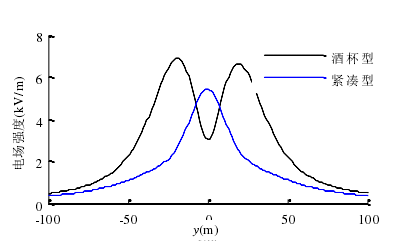
\includegraphics[width=8cm]{3.png}
\caption{电力塔周围的电场强度} 
\label{3}
\end{figure}


\subsection{特高压输电线路工频磁场分析}

当传输线工作时,电流周围产生磁场。有几个因素决定了磁场的强度,例如传输线的高度,传输线的布局等。与上面关于电场的分析有关,我们还关注传输线的布局和高度。

\subsubsection{传输线布局对磁场的影响}
	
由每个相传输线中的电流产生的磁场可以通过安培环定理直接获得,并且可以通过叠加由所有线产生的磁场来获得线周围的磁场强度。在陈伯东的论文“超高压输电线路电磁环境的数值模拟研究”中,考虑了镜像电流的影响,并通过镜像法计算了磁场强度。与电场的计算不同,磁场的计算考虑了传输线的下垂,这意味着线不能被认为是水平线。计算显示了传输线布局的影响。倒三角形布置使磁感应强度最小化,并且最大磁感应强度出现在线下方,如图4所示。基于该图,在电源结构中应考虑倒三角形布置。同样,不同的输电线路布局符合不同类型的塔架,以满足不同布局线路的需求。结果如上图所示,清楚地表明紧凑型塔的磁场强度低于杯型塔。它还可以反映紧凑型塔的优越性。
\begin{figure}[htbp]
\small
\centering
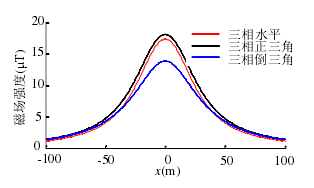
\includegraphics[width=8cm]{4.png}
\caption{传输线布局对磁场的影响} 
\label{4}
\end{figure}

\begin{figure}[htbp]
\small
\centering
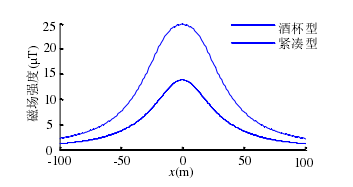
\includegraphics[width=8cm]{41.png}
\caption{传输线布局对磁场的影响2} 
\label{41}
\end{figure}

塔的类型2-D 3-D偏差

杯式塔25.64 24.68 3%

紧凑型塔13.83 13.95 0.8%

\subsubsection{传输线高度对磁场的影响}
	
传输线的高度会影响磁场,这与电场相似。在张可欣的论文中,他用Biot Savart定律计算了导线周围任意点的工频磁场和微积分的意识形态。任何电流,其中电流相当于大量微小的直流导线。传输线周围任何点的磁场都可以视为矢量,它是所有微小等效线的组合。具体计算在他的论文“超高压输电线路电磁环境研究(2009)”

\begin{figure}[htbp]
\small
\centering
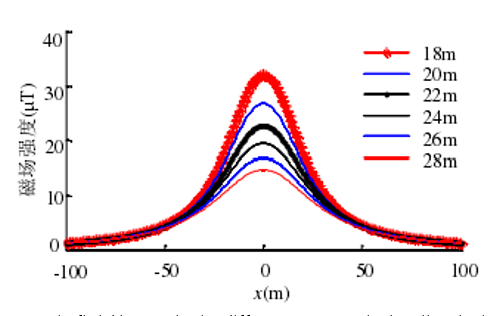
\includegraphics[width=8cm]{5.png}
\caption{传输线高度对磁场的影响} 
\label{5}
\end{figure}

结果清楚地显示在图~\ref{5}	中,这表明我们可以通过增加传输线的高度来降低地面磁场的强度。当高度达到一定值时,磁场衰减很慢,但在一定的高度范围内,通过改变线高可以有效地减小地面附近的磁场。结果激发了我们,在某种程度上,我们可以提高高度,以减少地面磁场的强度。如果我们需要进一步减少它,应该使用其他方法。然而,根据ICNIRP规则,磁场公开曝光的极限是100μT,这在很大程度上高于图5中的数据。因此,当涉及传输线产生的电磁场对人体健康的影响时,只应考虑电场。

\subsection{小结}
电磁环境与线路的高度,传输线的布局,不同线路之间的距离等有关,可以通过几种方法最小化。该方法包括提高输电线路的高度,选择理想的输电塔等。基本上,中国的电磁环境是1000kV的特高压交流输电线路是环保的。

尽管压实塔在电磁环境中具有比杯形塔更好的性能,但杯形塔可以满足各种对电磁环境的需求,而不管该区域的高度。但是,杯型塔的线路走廊宽度大于压实塔的走廊宽度。因此,在高度和线路走廊宽度方面,压实塔比杯形塔具有优势。压实塔的缺点也很明显---在2500m以上使用时不能满足无线电干扰58dB的限制要求,这只是一个无法弥补其优势的小缺陷。

我们可以在低海拔地区使用它来充分利用其经济效益。我们可以根据我们遇到的情况选择理想类型的塔,以充分利用每个塔的优势。


\section{减小工频电磁场影响的措施}

\subsection{降低工频电场强度的措施}

从目前我国的行业规范以及现场实测数据看,出于环保等原因,在某些情况下降低输电线路下方的工频电场是必须的。

除了本文中所述的选择合适的线路对地距离、相间距离以及相序等措施可以降低电场强度外,当线路投入运行后,可以采用在各相导线与地面之间架设屏蔽线的方法。需要指出的是屏蔽线根数的增加与场强的减小并不成比例,解决实际问题时,可以先用等效电荷法或模拟电荷法计算屏蔽效果,再从技术、经济和施工难度等多方面综合考虑,选择合适的屏蔽线的位置与数量。试验表明,在房顶采取架设接地围栏的方法也可以降低局部场强。

\subsection{降低工频磁场的措施}

从目前我国的行业规范以及现场实测数据看,工频磁场的环保指标比输电线下实际情况有较大裕度,很少需要采取专门的措施降低磁场强度。为减小输电线附近的工频磁场,可以在输电线附近架设平行于输电线路的架空屏蔽导线。

\section{缓解因输变电工程电磁环境所引起的环保问题的对策}

\begin{enumerate}

\item  输变电工程在规划、设计、建设和运行的各个阶段应严格按照相关法规、行业规范进行,并认真履行有关的环保程序,从而尽量避免因电磁环境问题而引起的纠纷并减小电力建设规划与城市建设规划的不同步性。
\item 规范测量手段,严格按照《高压交流架空送电线路、变电站工频电场和磁场测量方法》(DL/ T998 - 2006) 测量,对于确实超过有关环保标准或是行业标准的情况,应积极采取相应屏蔽措施。
\item 针对公众对输变电工程产生的电磁场的误解,电力部门和其他有关单位应加强科普宣传,正确引导公众理解工频电、磁场,尤其是与高频电磁辐射的区别,消除公众的担忧甚至恐慌。

\end{enumerate}

\section{工频电磁场的生态效应}

工频电场的生态效应,可分为短时影响和长期
影响(有的文献只将长期影响称为生态效应) 。
短时影响主要是指人体对电击和电场的直接
感受。较高的工频电场会使人有不舒服的感觉,这
种不舒服的感觉在瞬态放电时尤为明显。1 个绝缘
体(它有1 个“悬浮”电位) 与另1 个接地的或是与
带电设备有电气联系的物体,在稳定接触前的一瞬
间,若电位差足够大,就会产生1 个小电火花,此时
电流比稳态时高很多。在高压、超高压输电线下,
对地绝缘的人接触接地设备、接地的人接触绝缘的
设备等情况,如接触汽车、晒晾衣服的铁丝、雨伞等
金属物体,这种暂态放电的现象较易发生,同时会
伴有不同程度的刺痛感。这种暂态放电对人体造
成的不舒服程度除了和人与物之间的电位差有关
外,还与接触的部位、面积以及个人的心理、生理因
素有关。相比于持续时间大于几毫秒的电流通过
生物的影响已有相当准确的数据而言,国内外对持
续时间短的脉冲电流通过生物的影响的研究则十
分有限,虽有一些试验结果,但很难得到较为统一
的数据与研究结论。武汉高压研究所进行的触摸
尖顶金属伞杆的感受试验结果见表2 。一般认为,
在3 kV/ m 场强下,暂态电击是可以接受的。需要
指出的是,虽然在超高压输电线路地面附近有可能
存在每米几千伏的电场强度,因为人体内感应电流
很小(微安数量级) ,而且人体内部电阻较低(几百
欧姆) ,所以人体内部电场强度很少超过外部电场
强度的百万分之一。

 长期影响是指从生物学和病理学的角度来研
究人或动物甚至植物长期经常性的在高场强区的
反应,如行为表现、血象、生化指标、脏器病理变化
等。近30 a ,国际上关于工频电场的生物效应(尤
其是长期影响) 研究非常热烈,研究方法主要是基
于流行病学、动物实验和暴露量统计分析,所得出的
结论存在很大的非一致性。由于缺乏对工频电磁场
如何影响人体健康的基本机理的明确认识,尤其是微
观机理尚不清楚,至今还未得出确定性结论。


\section{工频电(磁) 场限值}

2002 年10 月通过的《中华人民共和国环境影
响评价法》,其中《建设项目环境保护管理办法》规
定,500 kV 以下输变电工程在敏感区要编制环境影
响报告书,500 kV 及以上,在非敏感区也要编制环
境影响报告表。关于高压送变电设备的工频电、磁
场限值目前尚无国家标准,但国家标准的研究工作
正在进行,且已经制订了“国标意见稿”。《500 kV
超高压送变电工程电磁辐射环境影响评价技术规
范》(HJ / T24 - 1998) 推荐以4 kV/ m 作为居民区工
频电场评价标准,推荐应用国际辐射保护协会制定
的对公众全天辐射时的工频限值0. 1 mT 作为磁感
应强度的评价标准。《110~500 kV 架空送电线路
设计技术规范》(DL/ T 5092 - 1999) 第16. 0. 5 条规
定:500 kV 送电线路跨越非长期住人的建筑物或邻
近民房时房屋所在位置离地1 m 处最大未畸变电
场不得超过4 kV/ m。到目前为止,还没有工频电
磁场暴露限值的IEC 标准或其它国际标准,只有国
际非电离辐射防护委员会( ICNIPRP) 向世界各国
推荐了1 个电磁场限值的导则。许多国家都有自
己的工频电磁场暴露(包括职业暴露与公众暴露)
标准,一些国际组织也建立了自己的导则作为各国
确定标准的建议。应该指出, ICNIPRP 的限值既考
虑了工频电磁场的短时效应也考虑了长期效应,是
在进行了充分实验的前提下提出的阈值,也是目前
世界上认可度比较高的限值标准。

对于工频电磁场的测量,应严格按照《高压交流
架空送电线路、变电站工频电场和磁场测量方法》
(DL/ T 998 - 2006) 进行,在解决由电磁环境问题引
发的纠纷时,这一点尤其重要。

\section{目前国家对于电磁环境的重视程度}
早在2005年国家电网论证特高压电网关键技术时,就单独考虑了电磁环境和对区域生态环境的影响。

国家电网公司对电磁环境问题高度重视,提出了建设环境友好型输电工程的目标,请国内外权威机构开展了深入研究,确立了保持交流特高压的电磁环境等影响指标限值与我国500kV 输电工程水平相当、特高压直流的电磁环境等影响指标限值与我国±500kV 输电工程水平相当的原则。特高压输电工程电磁环境的控制指标限值及工程环境评价报告已通过国家环保总局组织的审查。所确立的环境指标控制限值既能满足环保要求,又能以适当的造价在工程中实现。研究结论如下\cite{舒印彪20062005}:

\begin{enumerate}

\item 
只要设计合理,可使特高压输电工程的工频电场、工频磁场、合成场强、离子流强度和可听噪声水平与超高压输电工程的相当。
\item 
提出我国特高压输电线路的工频电场、工频磁场、合成场强、离子流强度和可听噪声的推荐限值。建议lOOOkV 级交流输电线路的工频电场和工频磁场的限值与我国500kV 交流输电线路的相同;可听噪声限值满足我国噪声标准要求。
\item 
工频电场、工频磁场、合成场强、离子流强度和可听噪声对人和某些动物有确定的有害影响的阐值远高于输电线路下的限值:特高压输电线路电磁环境有关量所取限值不会对人和动物造成有害影响。特高压输电线路工频电场和合成场强不会对线下农作物、植物和树木的生长带来不利影响。特高压输电线路对动物的迁徙、活动不会带来不利影响。在输送相同功率的条件下,与采用超高压输电相比,采用特高压输电占用土地少,对生态环境的影响面小。

\end{enumerate}

\section{结论}
交流输电线路对环境的影响从电磁角度分析,主要有工频电、磁场,无线电干扰,电晕噪声等.

电磁环境与线路的高度,传输线的布局,不同线路之间的距离等有关,可以通过几种方法最小化。该方法包括提高输电线路的高度,选择理想的输电塔等。基本上,中国的电磁环境是1000kV的特高压交流输电线路是环保的。


\section{致谢}

感谢老师的指导和队友的帮助~

%\section{附录}


%% 参考文献
% 注意:至少需要引用一篇参考文献,否则下面两行可能引起编译错误。
% 如果不需要参考文献,请将下面两行删除或注释掉。
% 数字式引用
\bibliographystyle{plain}
\bibliography{ref/refs}

\end{document}
